
\chapter{Statistica descrittiva}

Permette la rappresentazione dei dati in maniera chiara, precisa, concisa e sintetica.

Si utilizzano diversi tipi di grafici in base al contesto.

\section{Grandezze per sintetizzare i dati}

Si hanno $n$ dati.

\begin{equation}
  n : x_1, x_2, \dots, x_n
\end{equation}

L'ampiezza(numerosit\`{a}) dei dati sar\`{a} $n$.
\subsection{Centro dei dati}
\subsubsection{Media campionaria}
La media campionaria \`{e} una media pesata!

\begin{equation}
    \bar{x} = \displaystyle\frac{1}{n} \displaystyle\sum_{i = 1}^{n} x_i
\end{equation}

Dove la $n$ rappresenta il numero di elementi presi in considerazione per la media.

\subsubsection{Mediana campionaria}

Avendo un insieme di dati $n$ \textbf{ordinato}:
\begin{itemize}
    \item Se $n$ è dispari, la mediana campionaria è il valore in posizione $(n + 1) / 2$
    \item Se $n$ è pari, la mediana campionaria è la media dei valori in posizione $n / 2$ e $n / 2 + 1$
\end{itemize}


\subsubsection{Varianza} 
Avendo un'insieme di dati $x_1, x_2, \dots, x_n$, la varianza campionaria è:

\begin{equation}
    s^2 = \displaystyle\frac{1}{n - 1} \displaystyle\sum_{i = 1}^{n} (x_i - \bar{x})^2
\end{equation}

\subsubsection{Devizione standard} 
Avendo un'insieme di dati $x_1, x_2, \dots, x_n$, la deviazione standard è:

\begin{equation}
    s = \sqrt{\displaystyle\frac{1}{n - 1} \displaystyle\sum_{i = 1}^{n} (x_i - \bar{x})^2}
\end{equation}


\subsection{Percentili campionari}

\begin{figure}[!ht]
    \begin{center}
        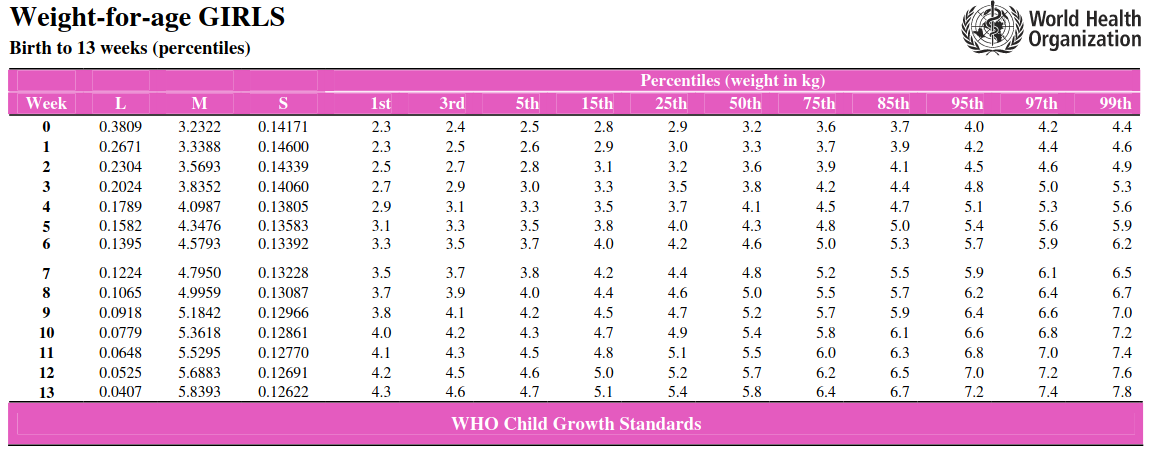
\includegraphics[width=0.8\textwidth]{./images/percentile_example.png}
    \end{center}
    \caption{Esempio percentili}
    \label{fig:esempio_percentili}
\end{figure}

Da questo graafico dell'OMS si capisce bene coasa sono i percentili. 

Le bambine che fanno parte del 25 esimo percentile hanno un peso alla nascita di $2.9$ Kg, 
il $25\%$ della bambine pesano meno e il $75\%$ delle bambine pesano di più. 

Il percentile divide i dati in due parti ben distinte, se il dato non è unico(due dati), si fa la media aritmetica. 

\subsubsection{Procedura}

Ho $n$ dati e voglio il valore del percentile k-esimo:
\begin{equation}
   p = \displaystyle\frac{k}{100} 
\end{equation}

\begin{equation}
   np = n \displaystyle\frac{k}{100} 
\end{equation}

Se $np$ non è intero, arrotondo al numero per eccesso successivo.



\subsubsection{Nota bene}
Sono quartili campionari: 
\begin{itemize}
    \item 25-esimo percentile
    \item 50-esimo percentile
    \item 75-esimo percentile
\end{itemize}

Notare che il 50-esimo percentile è la media campionaria.


\subsection{Box plot}
\begin{figure}[!ht]
    \begin{center}
        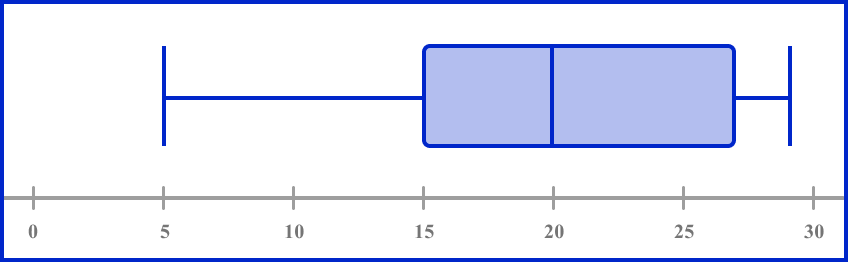
\includegraphics[width=0.5\textwidth]{./images/box_plot_example.png}
    \end{center}
    \caption{Esempio box plot}
    \label{fig:box_plot_example}
\end{figure}

Il disegno del box plot segue le seguenti regole:
\begin{itemize}
    \item linea da dato minore a dato maggiore
    \item box dal primo al terzo quartile
\end{itemize}

La lunghezza della linea rappresenta il campo di variazione(range dei valori), mentre la lunghezza del box 
rappresenta lo scarto interquartile. 

\section{Disuguaglianza di Chebyshev}
Avendo un'insieme di dati $x_1, x_2, \dots, x_n$ con media campionaria $\bar{x}$ e deviazione standard $s > 0$. 

Denoto con $S_k$ l'insieme degli indici dei dati compresi tra $\bar{x}-ks$ e $\bar{x}+ks$.

Essendo $\#S_k$ il numero di elementi dell'insieme $S_k$.(AKA cardinalità) 

Ne deriva la seguante equazione se $k \geq 0$:
\begin{equation}
   \displaystyle\frac{\#S_k}{n} \geq 1 - \displaystyle\frac{n - 1}{n k^2} > 1 - \displaystyle\frac{1}{k^2} 
\end{equation}


\section{Campioni normali}
Forma della distribuzione \textbf{caratteristica}:
\begin{itemize}
    \item a campana
    \item massimo sulla mediana
    \item simmetrica
\end{itemize}

Può essere approssimativamente normale o sbilanciata(skewed).


\subsection{Regola empirica}
\begin{itemize}
    \item Il $\sim 68\%$ dei dati si trova nella spazio $\bar{x} \pm s$
    \item Il $\sim 95\%$ dei dati si trova nella spazio $\bar{x} \pm 2s$
    \item Il $\sim 99.7\%$ dei dati si trova nella spazio $\bar{x} \pm 3s$
\end{itemize}


\section{Dati bivarianti}

Sono serie di dati diverrsi che hanno una correlazione fra di loro. 

La formula della correlazione è:
\begin{equation}
    (x_i - \bar{x})(y_i - \bar{y})
\end{equation}


Se il risultato è:
\begin{itemize}
    \item $> 0 \Rightarrow$ correlazione positiva
    \item $< 0 \Rightarrow$ correlazione negativa
\end{itemize}


\subsection{Coefficiente di correlazione campionaria}

\begin{equation}
   r = \displaystyle\frac{
        \displaystyle\sum_{i = 1}^{n} (x_i - \bar{x})(y_i - \bar{y})
   }{
        (n - 1)s_xs_y
   } 
\end{equation}


\begin{itemize}
    \item $r > 0 \Rightarrow$ correlazione positiva
    \item $r < 0 \Rightarrow$ correlazione negativa
\end{itemize}

\textbf{La correlazione è diversa dalla relazione di causa effetto.}


